\documentclass{article}
\usepackage{graphicx}
\usepackage{amsmath}
\DeclareMathOperator*{\argmin}{argmin}
\usepackage{hyperref}
\usepackage{titling}
\newcommand{\subtitle}[1]{%
  \posttitle{%
    \par\end{center}
    \begin{center}\large#1\end{center}
    \vskip0.5em}%
}
\title{Math 110A Project 1 Report}
\subtitle{Implementing Steepest Gradient Descent}
\author{by Alicia Chuang, Tyler Brown, Vinachau Pham}
\date{February 2023}

\begin{document}

\maketitle

\section{Steepest Gradient Descent}
The Steepest Gradient Descent Method is a first order optimization algorithm for finding local minimizers. Since the gradient is the direction of most positive change, any differentiable function decreases the fastest in the direction of the negative gradient. Thus, for an initial guess $\textbf{x}^{(0)}$, we can use the algorithm \[\textbf{x}^{(k+1)} = \textbf{x}^{(k)} - \alpha_k \nabla f(\textbf{x}^{(k)})\]
with $\alpha_k$ being the step size of each iteration, to approximate the local minimizer $\textbf{x}^{*}$. Convergence is reached once $\nabla f(\textbf{x}^{(k)})$ is within the tolerated region of 0, since $f(\textbf{x}^{*})=0$ by definition. The optimal $\alpha_k$ can be found by solving the one dimensional optimization problem \[\alpha_k = \argmin_{\alpha>0}f(\textbf{x}^{(k)}-\alpha f(\textbf{x}^{(k)}))\]

\section{Secant Method}
Newton's method is one of the fastest converging optimization algorithms, but it requires the second derivative. In the case that the second derivative is not analytically computable, we may approximate $f''(x^{(k)})$ with \[\frac{f'(\textbf{x}^{(k)})-f'(\textbf{x}^{(k-1)}}{\textbf{x}^{(k)}-\textbf{x}^{(k-1)}}\]
Then, from the Newton's Method, we obtain the algorithm for the Secant Method: \[\textbf{x}^{(k+1)} = \textbf{x}^{(k)} - \frac{\textbf{x}^{(k)}-\textbf{x}^{(k-1)}}{f'(\textbf{x}^{(k)})-f'(\textbf{x}^{(k-1)})}f'(\textbf{x}^{(k)})\]


\section{Code and Output}
Our code is written in python, with comments, on this \href{https://github.com/AliciaChuang/MATH-110A-Project-1/blob/main/project.py}{github repository}
\bigskip

Testing only the linesearch\textunderscore secant function using $\alpha^2 - 20$ with initial guesses of $\alpha_0 = 2$ and $\alpha_1 = 8$, converging in 7 steps as expected:
\bigskip

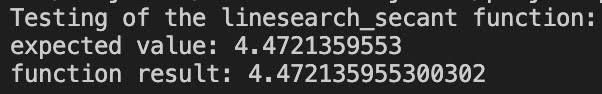
\includegraphics[scale=0.5]{linesearch.jpeg}

\bigskip

Testing the Rosenbrock's function $f(\textbf{x}) = 100*(\textbf{x}_1-\textbf{x}_0^2)^2+(1-\textbf{x}_0)^2$, 

with 
$\nabla f(\textbf{x}) = \begin{bmatrix}
400*\textbf{x}_0^3 - 400*\textbf{x}_0*\textbf{x}_1 + 2*\textbf{x}_0 - 2 \\
200*(\textbf{x}_1 - \textbf{x}_0^2)
\end{bmatrix}$, initial guess $\begin{bmatrix}
    1.5 \\
    2
\end{bmatrix}$, tolerance $10^{-9}$, initial guess $\alpha_0=0.01$ and $\alpha_1=0.011$, printing out every 20:

\bigskip

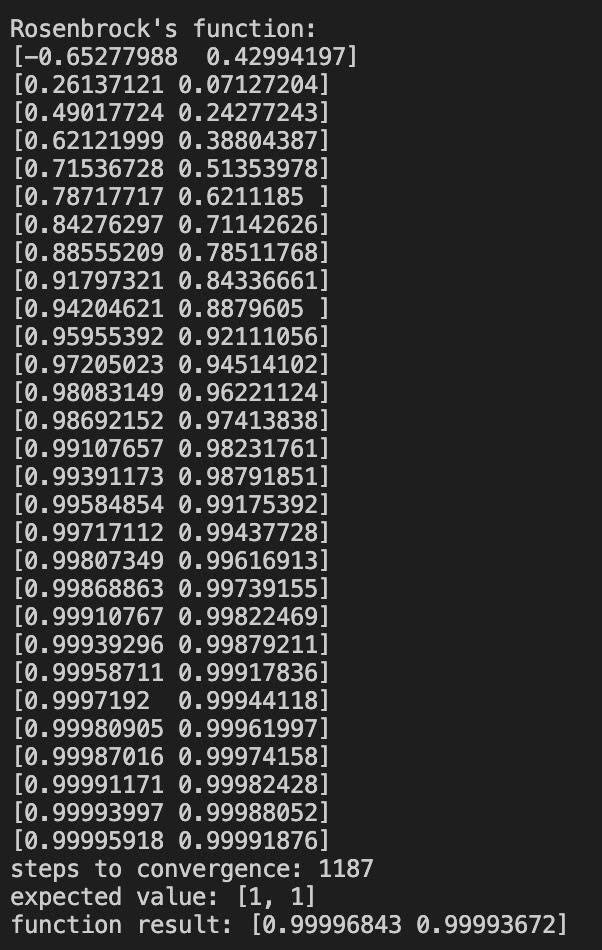
\includegraphics[scale=0.35]{rosennbrock's.jpeg}

\bigskip

Testing on the paraboloid $f(\textbf{x}) = \textbf{x}_0^2 + \textbf{x}_1^2$ with initial guess $\begin{bmatrix}
    10 \\
    12
\end{bmatrix}$, tolerance $10^{-9}$, initial guess $\alpha_0=1$ and $\alpha_1=1.5$:

\bigskip

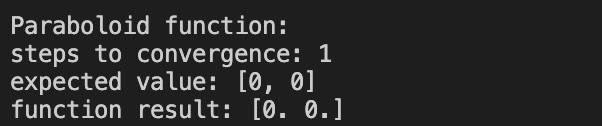
\includegraphics[scale=0.5]{paraboloid.jpeg}

\bigskip


\section{Analysis and Conclusion}
The algorithm works as expected, however, the parameters are not well suited to the Rosenbrock's function shape. Thus, the secant method takes a long time to converge using our initial guess.

\end{document}